%\documentclass[12pt]{article}
\documentclass[final, 12pt]{colt2018}
%\usepackage{fullpage}
\usepackage{hyperref}
%\usepackage{amsthm, amsmath, amsfonts, amssymb}
\usepackage{bbm}
\usepackage{cases}
\usepackage{graphicx}
\usepackage{pagecolor}
\usepackage{caption}
\usepackage{subcaption}
%\usepackage{cite}
\usepackage{mathtools}
\usepackage{verbatim}
%\usepackage{natbib}
%\bibliographystyle{plainnat}
%\usepackage{authblk}

% Convert to grayscale:
% gs -o name.pdf -sDEVICE=pdfwrite -sColorConversionStrategy=Gray  name.pdf

\tolerance=10000

\newtheorem{prop}{Proposition}
%\newtheorem{theorem}{Theorem}
%\newtheorem{corol}{Corollary}
%\newtheorem{lemma}{Lemma}

\newcommand{\footremember}[2]{%
    \footnote{#2}
    \newcounter{#1}
    \setcounter{#1}{\value{footnote}}%
}
\newcommand{\footrecall}[1]{%
    \footnotemark[\value{#1}]%
} 

\renewcommand{\theparagraph}{\arabic{section}.\arabic{subsection}.\arabic{paragraph}}
\setcounter{secnumdepth}{4}

\DeclareMathOperator*{\esssup}{ess\,sup}
\newcommand{\Mod}[1]{\ (\mathrm{mod}\ #1)}

\graphicspath{{./figs/}}

\begin{document}
\title{Optimal approximation of continuous functions by very deep ReLU networks
}
\coltauthor{\Name{Dmitry Yarotsky} \Email{d.yarotsky@skoltech.ru}\\
 \addr Skolkovo Institute of Science and Technology, Skolkovo Innovation Center, 3 Nobel st., Moscow  143026, Russia
 \and
 \addr Institute for Information Transmission Problems, Bolshoy Karetny per. 19, build.1, Moscow 127051, Russia
 }
% \author{Dmitry Yarotsky\footremember{skoltech}{Skolkovo Institute of Science and Technology, Skolkovo Innovation Center, Building 3, Moscow  143026
% Russia}\footremember{iitp}{Institute for Information Transmission Problems, Bolshoy Karetny per. 19, build.1, Moscow 127051, Russia}\\
% \texttt{d.yarotsky@skoltech.ru}
% }
% \date{}
\maketitle


\begin{abstract} We consider approximations of general continuous functions on finite-dimensional cubes by general deep ReLU neural networks and study the approximation rates with respect to the modulus of continuity of the function and the total number of weights $W$ in the network. We establish the complete phase diagram of feasible approximation rates and show that it includes two distinct phases. One phase corresponds to slower approximations that can be achieved with constant-depth networks and continuous weight assignments. The other phase provides faster approximations at the cost of depths necessarily growing as a power law $L\sim W^{\alpha}, 0<\alpha\le 1,$ and with necessarily discontinuous weight assignments. In particular, we prove that constant-width fully-connected networks of depth $L\sim W$ provide the fastest possible approximation rate $\|f-\widetilde f\|_\infty = O(\omega_f(O(W^{-2/\nu})))$ that cannot be achieved with less deep networks.\footnote{Extended abstract.
The full version with the proofs appears as [arXiv:1802.03620, v2]}  
\end{abstract}

\section{Introduction}
Expressiveness of deep neural networks with piecewise-linear (in particular, ReLU) activation functions has been a topic of much theoretical research in recent years. The topic has many aspects, with connections to combinatorics \citep{montufar2014number,telgarsky2016benefits}, topology \citep{bianchini2014complexity}, Vapnik-Chervonenkis dimension \citep{bartlett1998almost,sakurai1999tight} and fat-shattering dimension \citep{kearns1990efficient,anthony2009neural}, hierarchical decompositions of functions \citep{mhaskar2016learning}, information theory \citep{petersen2017optimal}, etc.

Here we adopt the perspective of classical approximation theory, in which the problem of expressiveness can be basically described as follows. Suppose that $f$ is a multivariate function, say on the cube $[0,1]^\nu$, and has some prescribed regularity properties; how efficiently can one approximate $f$ by deep neural networks?  The question has been studied in several recent publications. Depth-separation results for some explicit families of functions have been obtained in \cite{safran2016depth, telgarsky2016benefits}. General upper and lower bounds on approximation rates for functions characterized by their degree of smoothness have been obtained in \cite{liang2016why, yarotsky2017nn}. \cite{hanin2017approximating, lu2017expressive} establish the universal approximation property and convergence rates for deep and ``narrow'' (fixed-width) networks. \cite{petersen2017optimal} establish convergence rates for approximations of discontinuous functions. Generalization capabilities of deep ReLU networks trained on finite noisy samples are studied in \cite{schmidthieber2017nonparametric}.

In the present paper we consider and largely resolve the following  question: what is the optimal rate of approximation of general continuous functions by deep ReLU networks, in terms of the number $W$ of network weights and the modulus of continuity of the function? Specifically, for any $W$ we seek a network architecture with $W$ weights so that for any continuous $f:[0,1]^\nu\to \mathbb R$, as $W$ increases, we would achieve the best convergence in the uniform  norm $\|\cdot\|_\infty$ when using these architectures to approximate $f$.

In the slightly different but closely related context of approximation on balls in Sobolev spaces $\mathcal W^{d,\infty}([0,1]^\nu),$ this question of optimal convergence rate has been studied in \cite{yarotsky2017nn}. That paper described ReLU network architectures with $W$ weights ensuring approximation with error $O(W^{-d/\nu}\ln^{d/\nu} W)$ (Theorem 1). The construction was linear in the sense that the network weights depended on the approximated function linearly. Up to the logarithmic factor, this approximation rate matches the optimal rate over all parametric models under assumption of continuous parameter selection (\cite{devore1989optimal}). It was also shown in Theorem 2 of \cite{yarotsky2017nn} that one can slightly (by a logarithmic factor) improve over this conditionally optimal rate by adjusting network architectures to the approximated function.  

On the other hand, it was proved in Theorem 4 of \cite{yarotsky2017nn}  that ReLU networks generally cannot provide approximation with accuracy better than $O(W^{-2d/\nu})$ -- a bound with the power $\frac{2d}{\nu}$ twice as big as in the previously mentioned existence result. As was shown in the same theorem, this bound can be strengthened for shallow networks. However, without imposing depth constraints, there was a serious gap between the powers $\frac{2d}{\nu}$ and $\frac{d}{\nu}$ in the lower and upper accuracy bounds that was left open in that paper.

In the present paper we bridge this gap in the setting of continuous functions (which is slightly more general than the setting of the Sobolev space of Lipschitz functions, $\mathcal W^{1,\infty}([0,1]^\nu)$, i.e. the case $d=1$). Our key insight is the close connection between approximation theory and VC dimension bounds. The lower bound on the approximation accuracy in Theorem 4 of \cite{yarotsky2017nn} was derived using the upper VCdim bound $O(W^2)$ from \cite{goldberg1995bounding}. More accurate upper and lower bounds involving the network depth $L$ have been given in \cite{bartlett1998almost,sakurai1999tight}. The recent paper \cite{bartlett2017nearly} establishes nearly tight lower and upper VCdim bounds: $cWL\ln (W/L)\le\operatorname{VCdim}(W,L)\le CWL\ln W$, where $\operatorname{VCdim}(W,L)$ is the largest VC dimension
of a piecewise linear network with $W$ weights and $L$ layers. The key element in the proof of the lower bound is the ``bit extraction technique'' (\cite{bartlett1998almost}) providing a way to compress significant expressiveness in a single network weight.  In the present paper we adapt this technique to the approximation theory setting.

Our main result is the complete phase diagram for the parameterized family of approximation rates involving the modulus of continuity $\omega_f$ of the function $f$ and the number of weights $W$. We prove that using very deep networks one can approximate function $f$ with error $O(\omega_f(O(W^{-2/\nu})))$, and this  rate is optimal up to a logarithmic factor. In fact, the depth of the networks must necessarily grow almost linearly with $W$ to achieve this rate, in sharp contrast to  shallow networks that can provide approximation with error $O(\omega_f(O(W^{-1/\nu})))$. Moreover, whereas the slower rate $O(\omega_f(O(W^{-1/\nu})))$ can be achieved using a continuous weight assignment in the network, the optimal $O(\omega_f(O(W^{-2/\nu})))$ rate necessarily requires a discontinuous weight assignment. All this allows us to regard these two kinds of approximations as being in different ``phases''. In addition, we explore the intermediate rates $O(\omega_f(O(W^{-p})))$ with $p\in(\frac{1}{\nu},\frac{2}{\nu})$ and show that they are also in the discontinuous phase and require network depths $\sim W^{p\nu-1}.$ We show that the optimal rate $O(\omega_f(O(W^{-2/\nu})))$ can be achieved with a deep constant-width fully-connected architecture, whereas the rates $O(\omega_f(O(W^{-p})))$ with $p\in(\frac{1}{\nu},\frac{2}{\nu})$ and depth $O(W^{p\nu-1})$ can be achieved by stacking the deep constant-width architecture with a shallow parallel architecture.  Apart from the bit extraction technique, we use the idea of the two-scales expansion from Theorem 2 in \cite{yarotsky2017nn} as an essential tool in the proofs of our results.
 

\section{The results}\label{sec:result}
We define the modulus of continuity $\omega_f$ of a function $f:[0,1]^\nu\to\mathbb R$ by \begin{equation}\label{eq:omega}\omega_f(r)=\max\{|f(\mathbf x)-f(\mathbf y)|: \mathbf x, \mathbf y\in [0,1]^\nu, |\mathbf x-\mathbf y|\le r\},\end{equation}
where $|\mathbf x|$ is the euclidean norm of $\mathbf x$. 

%\pagecolor{yellow!30!orange}
\begin{figure}
\begin{center}
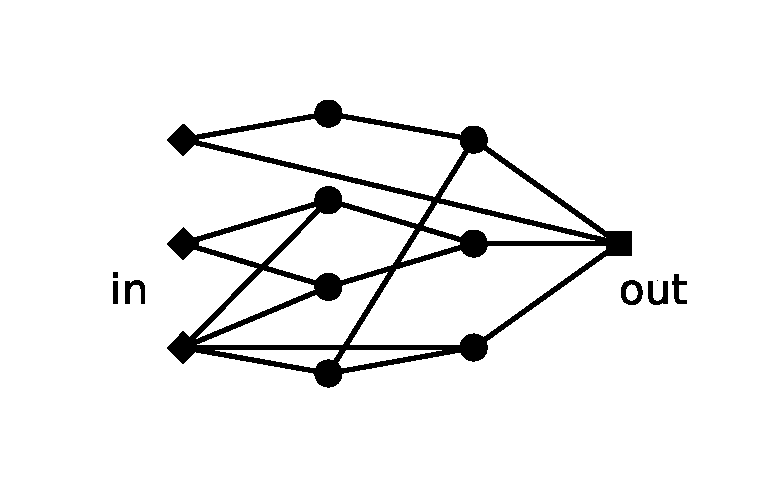
\includegraphics[clip,trim=12mm 8mm 12mm 8mm, scale=0.5]{netGray.eps}
\caption{An example of a feed-forward network architecture of depth $L=2$ with $W=24$ weights.}\label{fig:net}
\end{center}
\end{figure}

We approximate functions $f:[0,1]^\nu\to\mathbb R$ by usual feed-forward neural networks with the ReLU activation function $x\mapsto x_+\equiv \max(0,x)$.  The network has $\nu$ input units, some hidden units, and one output unit. The hidden units are assumed to be grouped in a sequence of layers so that the inputs of each unit is formed by outputs of some units from previous layers. The depth $L$ of the network is the number of these hidden layers. A hidden unit computes a linear combination of its inputs followed by the activation function: $x_1,\ldots,x_s\mapsto (\sum_{k=1}^s w_k x_k+h)_+$, where $w_k$ and $h$ are the weights associated with this unit. The output unit acts similarly, but without the activation function: $x_1,\ldots,x_s\mapsto \sum_{k=1}^s w_k x_k+h$. 

The network is determined by its architecture and weights. Clearly, the total number of weights, denoted by $W$, is equal to the total number of connections and computation units (not counting the input units). We don't impose any constraints on the network architecture (see Fig. \ref{fig:net} for an example of a valid architecture). 

Throughout the paper, we consider the input dimension $\nu$ as fixed. Accordingly, by \emph{constants} we will generally mean values that may depend on $\nu$.

We are interested in relating the approximation errors to the complexity of the function $f$, measured by its modulus of continuity $\omega_f$, and to the complexity of the approximating network, measured by its total number of weights $W$. More precisely, we consider  approximation rates in terms of the following procedure. 

First, suppose that for each $W$ we choose in some way a network architecture $\eta_W$ with $\nu$ inputs and $W$ weights. Then, for any $f:[0,1]^\nu\to\mathbb R$ we construct an approximation $\widetilde f_W:[0,1]^\nu\to \mathbb R$ to $f$ by choosing in some way the values of the weights in the architecture $\eta_W$  -- in the sequel, we refer to this stage as the \emph{weight assignment}. The question we ask is this: for which powers $p\in\mathbb R$ can we ensure, by the choice of the architecture and then the weights, that
\begin{equation}\label{eq:mainineq}
\|f-\widetilde f_W\|_\infty\le a\omega_f(c W^{-p}), \quad \forall f\in C([0,1]^\nu),
\end{equation}
with some constants $a, c$ possibly depending on $\nu$ and $p$ but not on $W$ or $f$?

Clearly, if inequality \eqref{eq:mainineq} holds for some $p$, then it also holds for any smaller $p$. However, we expect that for smaller $p$ the inequality can be in some sense easier to satisfy. In this paper we show that there is in fact a  \emph{qualitative} difference between different regions of $p$'s. 

%\pagecolor{yellow!30!orange}
\begin{figure}
\begin{center}
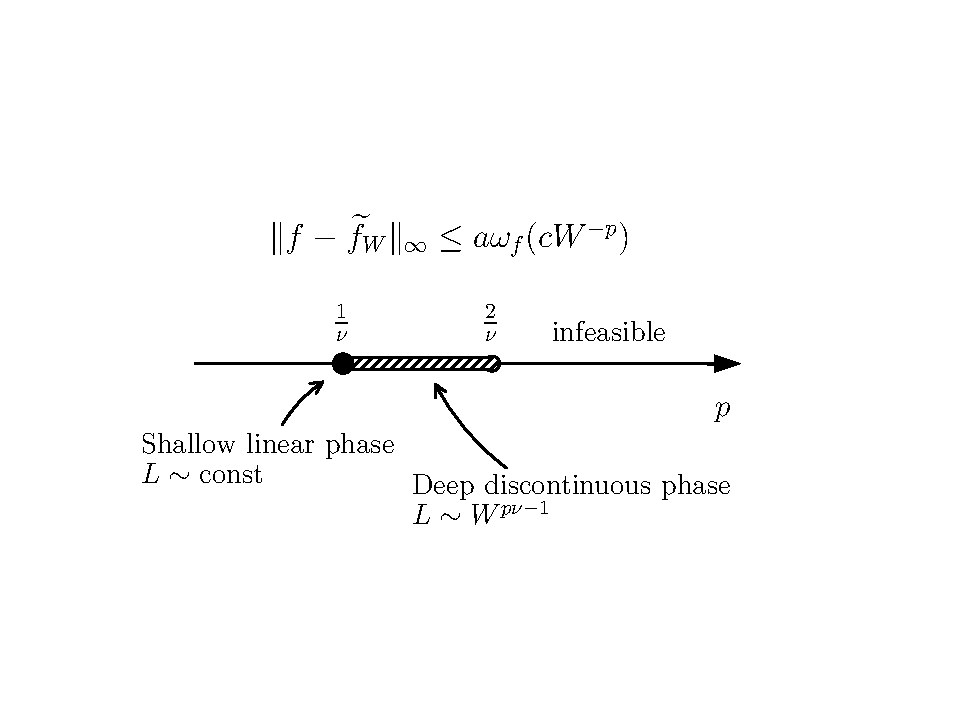
\includegraphics[clip,trim=20mm 30mm 30mm 35mm, scale=0.8]{phaseDiag_noType3fonts.pdf}
\caption{The phase diagram of convergence rates. At $p=\frac{1}{\nu}$ the rate is achieved by shallow networks with weights linearly (and continuously) depending on $f$. At $p\in(\frac{1}{\nu},\frac{2}{\nu}]$, the rate is achieved by deep networks with weights discontinuously depending on $f$. Rates with $p>\frac{2}{\nu}$ are infeasible.}\label{fig:phasediag}
\end{center}
\end{figure}

Our findings are best summarized by the phase diagram shown in Fig. \ref{fig:phasediag}. We give an informal overview of the diagram before moving on to precise statements. The region of generally feasible rates is $p\le \frac{2}{\nu}.$ This region includes two qualitatively distinct phases corresponding to $p=\frac{1}{\nu}$ and $p\in (\frac{1}{\nu}, \frac{2}{\nu}]$. At $p=\frac{1}{\nu},$ the rate \eqref{eq:mainineq} can be achieved by fixed-depth networks whose weights depend linearly on the approximated function $f$. In contrast, at $p\in (\frac{1}{\nu}, \frac{2}{\nu}]$ the rate can only be achieved by networks with growing depths $L\sim W^{p\nu-1}$ and whose weights depend \emph{discontinuously} on the approximated function. In particular, at the rightmost feasible point $p=\frac{2}{\nu}$ the approximating architectures have $L\sim W$ and are thus necessarily extremely deep and narrow. 

%\pagecolor{yellow!30!orange}
\begin{figure}[t]
\begin{center}
%\begin{subfigure}[b]{0.3\textwidth}
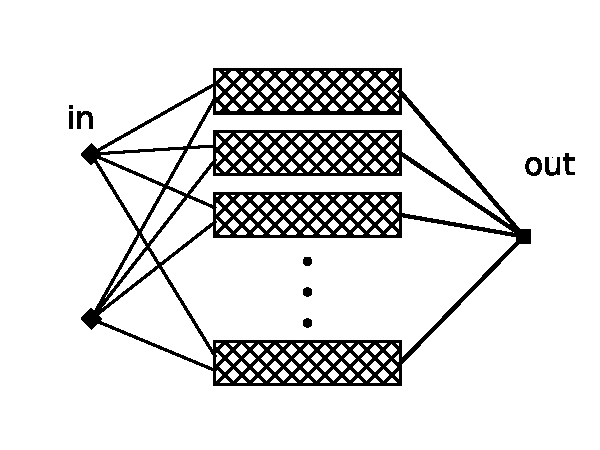
\includegraphics[clip,trim=5mm 10mm 0mm 10mm, scale=0.8]{shallowNet.pdf}
\caption{The parallel, constant-depth network architecture implementing piecewise linear interpolation and ensuring approximation rate \eqref{eq:mainineq} with $p=\frac{1}{\nu}$.}\label{fig:shallow}
%\end{subfigure}
%\begin{subfigure}[b]{0.3\textwidth}
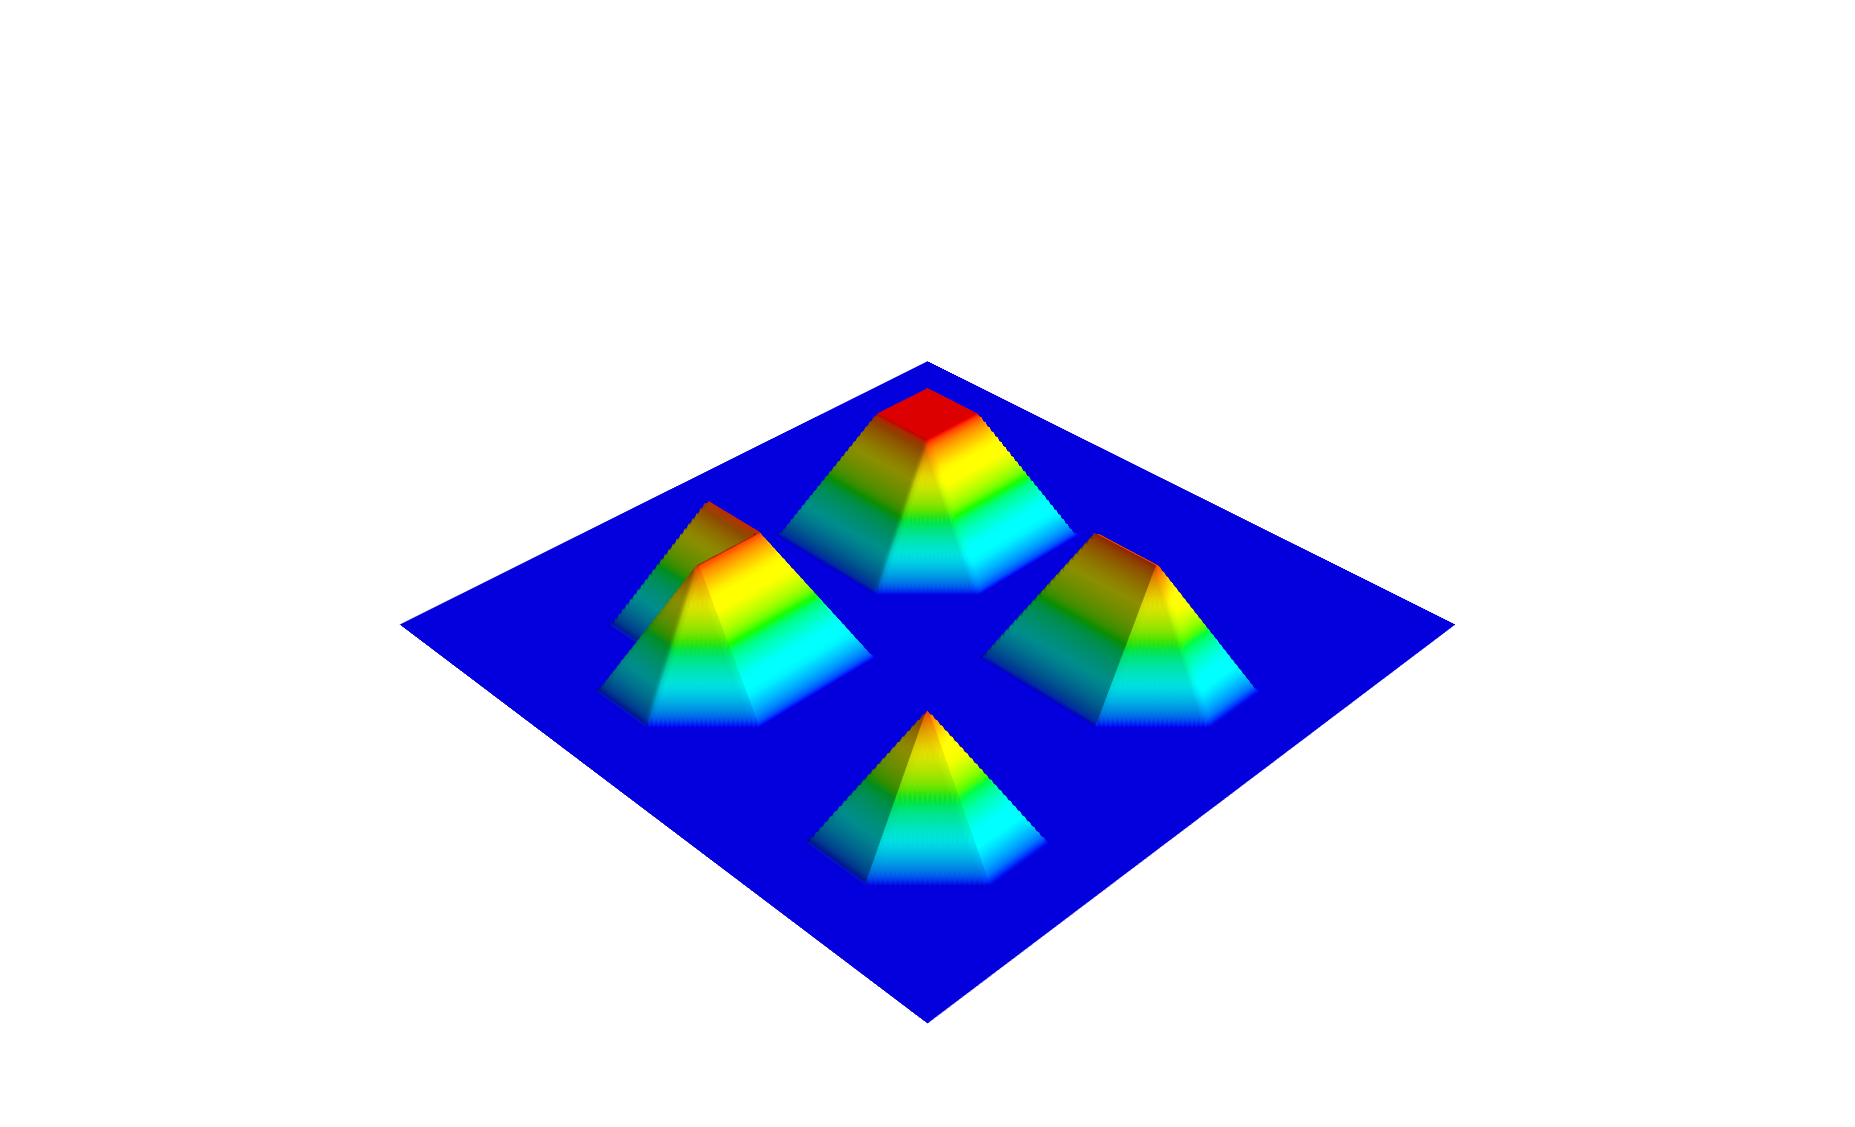
\includegraphics[clip,trim=120mm 30mm 120mm 105mm, scale=0.15]{spikes_lin4.png}
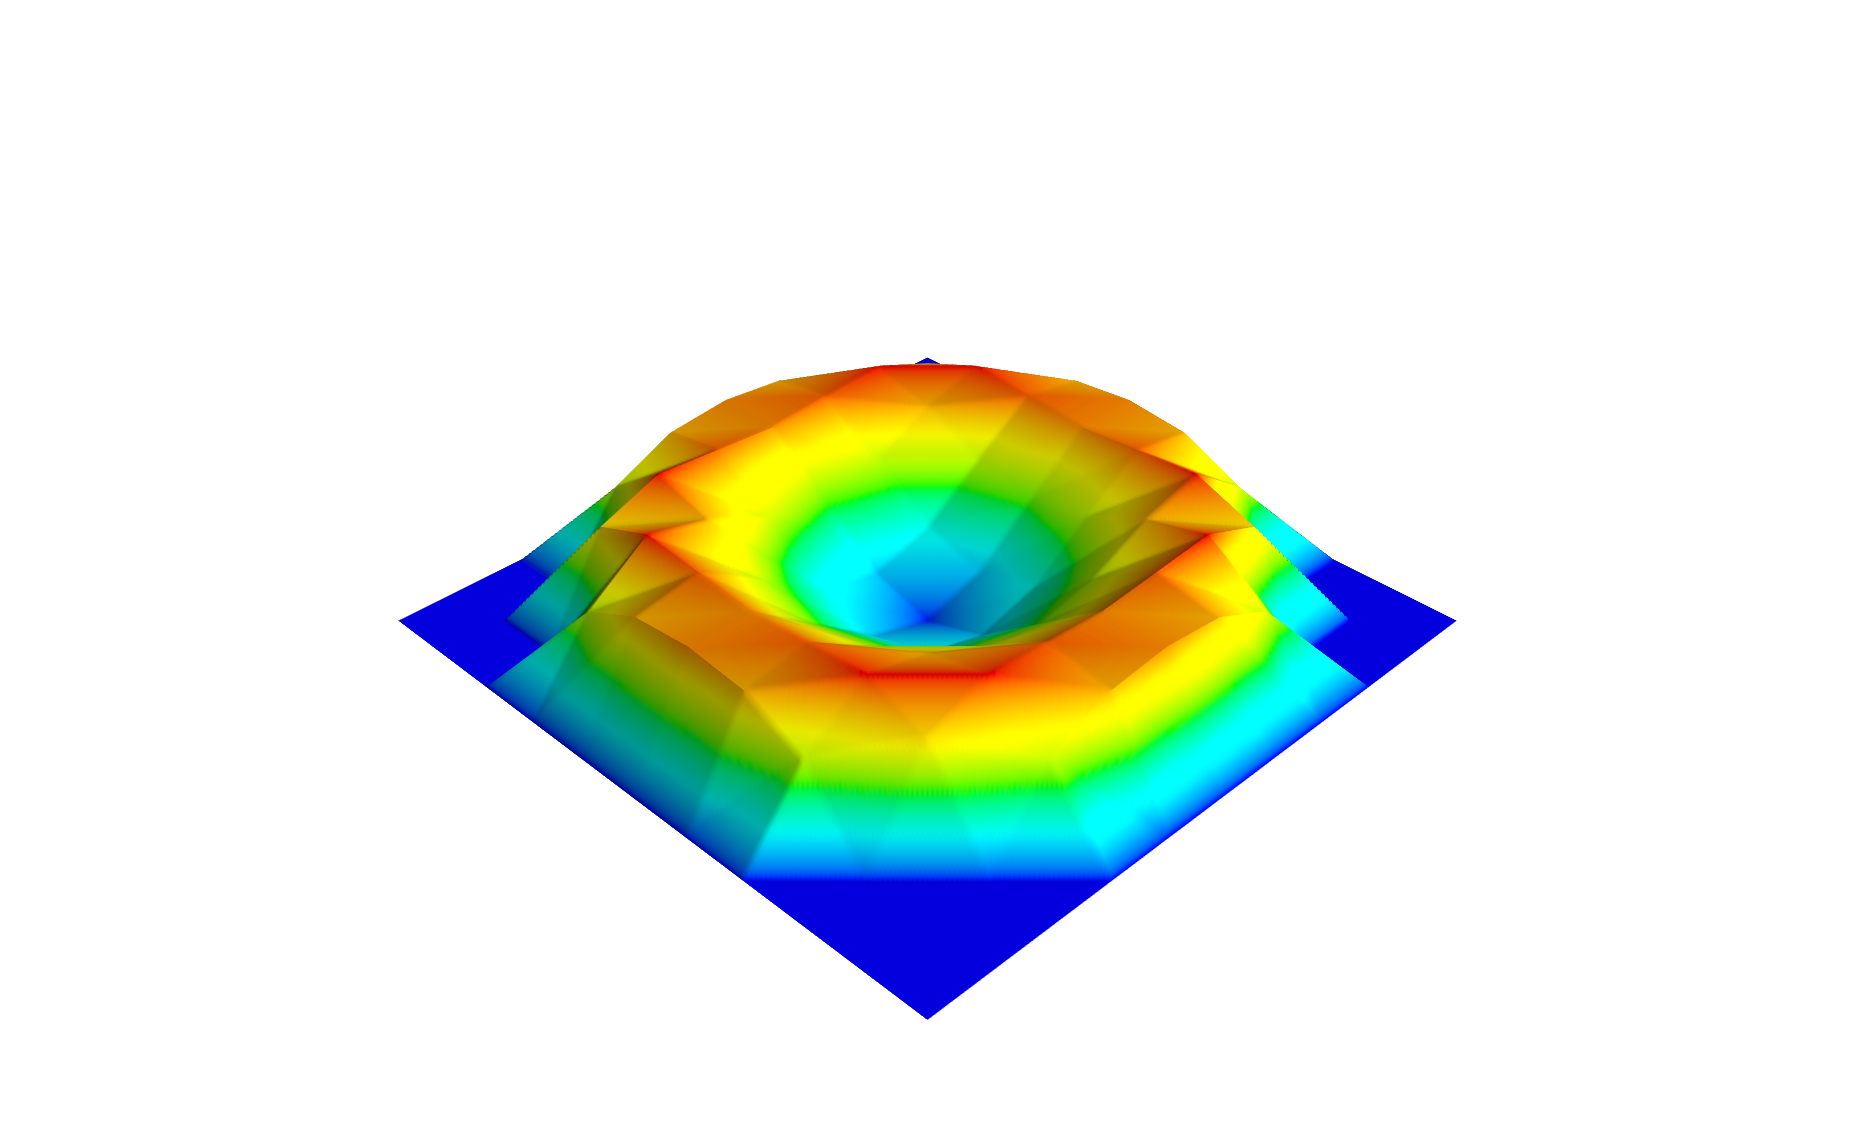
\includegraphics[clip,trim=120mm 30mm 120mm 125mm, scale=0.15]{spikes_lin5.png}
\caption{Approximation by linear combinations of ``spike'' functions in dimension $\nu=2$. Left: a spike function and examples of sums of neighboring spike functions. Right: approximation of a radial function by a linear combination of spike functions.}\label{fig:spikes}
%\end{subfigure}
\end{center}
\end{figure}

We now turn to precise statements. First we characterize the $p=\frac{1}{\nu}$ phase in which the approximation can be obtained using a standard piecewise linear interpolation. In the sequel, when writing $f=O(g)$ we mean that $|f|\le c g$ with some constant $c$ that may depend on $\nu.$  For brevity, we will write $\widetilde f$ without the subscript $W$.  

\begin{prop}\label{prop:shallow} There exist network architectures $\eta_W$ with $W$ weights and, for each $W$, a weight assignment linear in $f$ such that Eq. \eqref{eq:mainineq} is satisfied with $p=\frac{1}{\nu}.$  
The network architectures can be chosen as consisting of $O(W)$ parallel blocks each having the same architecture that only depends on $\nu$ (see Fig. \ref{fig:shallow}). In particular, the depths of the networks depend on $\nu$ but not on $W$. 
\end{prop}
We explain now the idea of the proof. The approximating function $\widetilde f$ is constructed as a linear combination of ``spike'' functions sitting at the knots of the regular grid in $[0,1]^\nu$, with coefficients given by the values of $f$ at these knots (see Fig. \ref{fig:spikes}). For a grid of spacing $\frac{1}{N}$ with an appropriate $N$, the number of knots is $\sim N^\nu$ while the approximation error is $O( \omega_f(O(\frac{1}{N}))).$ We implement each spike by a block in the network, and implement the whole approximation by summing blocks connected in parallel and weighted. Then the whole network has $O(N^\nu)$ weights and, by expressing $N$ as $\sim W^{1/\nu}$, the approximation error is $O(\omega_f(O(W^{-1/\nu}))$, i.e. we obtain the rate \eqref{eq:mainineq} with $p=\frac{1}{\nu}$.

We note that the weights of the resulting network either do not depend on $f$ at all or are given by $w=f(\mathbf x)$ with some $\mathbf x\in [0,1]^\nu.$ In particular, the weight assignment is continuous in $f$ with respect to the standard topology of $C([0,1]^\nu)$.   

We turn now to the region $p>\frac{1}{\nu}.$ Several properties of this region are either direct consequences or slight modifications of existing results, and it is convenient to combine them in a single theorem.

\begin{theorem}\label{th:2}{}\hfill
\begin{enumerate}
\item[a)] (Feasibility) Approximation rate \eqref{eq:mainineq} cannot be achieved with $p>\frac{2}{\nu}$.
\item[b)] (Inherent discontinuity) Approximation rate \eqref{eq:mainineq} cannot be achieved with $p>\frac{1}{\nu}$ if the weights of $\widetilde f$ are required to depend on $f$ continuously with respect to the standard topology of $C([0,1]^\nu)$.
\item[c)] (Inherent depth) If approximation rate \eqref{eq:mainineq} is achieved with a particular $p\in (\frac{1}{\nu},\frac{2}{\nu}]$, then the architectures $\eta_W$ must have depths $L\ge d W^{p\nu-1}/\ln W$  with some possibly $\nu$- and $p$-dependent constant $d>0.$
\end{enumerate}
\end{theorem}
\begin{proof} 
The proofs of these statements have the common element of considering the approximation for functions from the unit ball $F_{\nu,1}$ in the  Sobolev space  $\mathcal W^{1,\infty}([0,1]^\nu)$  of Lipschitz functions. Namely, suppose that the approximation rate \eqref{eq:mainineq} holds with some $p$. Then all $f\in F_{\nu,1}$ can be approximated by architectures $\eta_W$ with accuracy \begin{equation}\label{eq:epsw}\epsilon_W= c_1 W^{-p}\end{equation} with some constant $c_1$ independent of $W$. The three statements of the theorem are then obtained as follows.

\medskip\noindent
a) This statement is a consequence of Theorem 4a) of \cite{yarotsky2017nn}, which is in turn a consequence of the upper bound $O(W^2)$ for the VC dimension of a ReLU network (\cite{goldberg1995bounding}). Precisely, Theorem 4a) implies that if an architecture $\eta_W$ allows to approximate all $f\in F_{\nu,1}$ with accuracy $\epsilon_W$, then $W\ge c_2\epsilon_W^{-\nu/2}$ with some $c_2$. Comparing this with Eq. \eqref{eq:epsw}, we get $p\le \frac{2}{\nu}.$

\medskip\noindent 
b) This statement is a consequence of the general bound of \cite{devore1989optimal} on the efficiency of approximation of Sobolev balls with parametric models having parameters continuously depending on the approximated function. Namely, if the weights of the networks $\eta_W$ depend on $f\in F_{\nu,1}$ continuously, then Theorem 4.2 of \cite{devore1989optimal} implies that $\epsilon_W\ge c_2 W^{-1/\nu} $ with some constant $c_2$, which implies that $p\le\frac{1}{\nu}.$

\medskip\noindent 
c) This statement can be obtained by combining arguments of Theorem 4 of \cite{yarotsky2017nn} with the recently established tight upper bound for the VC dimension of ReLU networks (\cite{bartlett2017nearly}, Theorem 6) with given depth $L$ and the number of weights $W$: \begin{equation}\label{eq:vcub}\operatorname{VCdim}(W,L)\le CWL\ln W,\end{equation} where $C$ is a global constant. 

Specifically, suppose that an architecture $\eta_W$ allows to approximate all $f\in F_{\nu,1}$ with accuracy $\epsilon_W$. Then, by considering suitable trial functions, one shows that if we threshold the network output, the resulting networks must have VC dimension $\mathrm{VCdim}(\eta_W)\ge c_2\epsilon_W^{-\nu}$ (see Eq.(38) in \cite{yarotsky2017nn}). Hence, by Eq. \eqref{eq:epsw}, $\mathrm{VCdim}(\eta_W)\ge c_3 W^{p\nu}$. On the other hand,  the upper bound \eqref{eq:vcub} implies $\mathrm{VCdim}(\eta_W)\le CWL\ln W$. We conclude that $c_3W^{p\nu}\le CWL\ln W$, i.e. $L\ge dW^{p\nu-1}/\ln W$ with some constant $d$. 
\end{proof}

Theorem \ref{th:2} suggests the existence of an approximation phase drastically different from the phase $p=\frac{1}{\nu}$. This new phase would provide better approximation rates, up to $p=\frac{2}{\nu}$, at the cost of deeper networks and some complex, discontinuous weight assignment. The main contribution of the present paper is the proof that this phase indeed exists. 

We describe some architectures that, as we will show, correspond to this phase. First we describe the architecture for $p=\frac{2}{\nu},$ i.e. for the fastest possible approximation rate. Consider the usual fully-connected architecture connecting neighboring layers and having a constant number of neurons in each layer, see Fig. \ref{fig:stnet}. We refer to this constant number of neurons as the  ``width'' $H$ of the network. Such a network of width $H$ and depth $L$ has $W=L(H^2+H)+H^2+(\nu+1)H+1$ weights in total. We will be interested in the scenario of ``narrow'' networks where $H$ is fixed and the network grows by increasing $L$; then $W$ grows linearly with $L$. Below we will refer to the ``narrow fully-connected architecture of width $H$ having $W$ weights'': the depth $L$ is supposed in this case to be determined from the above equality; we will assume without loss of generality that  the equality is satisfied with an integer $L$. We will show that these narrow architectures provide the $p=\frac{2}{\nu}$ approximation rate if the width $H$ is large enough (say, $H=2\nu+10$).   

In the case $p\in (\frac{1}{\nu},\frac{2}{\nu})$ we consider another kind of architectures obtained by stacking parallel shallow architectures (akin to those of Proposition \ref{prop:shallow}) with the above narrow fully-connected architectures, see Fig. \ref{fig:stackednet}. The first, parallelized part of these architectures consists of blocks that only depend on $\nu$ (but not on $W$ or $p$). The second, narrow fully-connected part will again have a fixed width,  and we will take its depth to be $\sim W^{p\nu-1}$. All the remaining weights then go into the first parallel subnetwork, which in particular determines the number of blocks in it. Since the blocks are parallel and their architectures do not depend on $W$, the overall depth of the network is determined by the second, deep subnetwork and is $O(W^{p\nu-1})$. On the other hand, in terms of the number of weights, for $p<\frac{2}{\nu}$ most computation is performed by the first, parallel subnetwork (the deep subnetwork has $O(W^{p\nu-1})$ weights while the parallel one has an asymptotically larger number of weights, $W-O(W^{p\nu-1})$). 

Clearly, these stacked architectures can be said to ``interpolate'' between the purely parallel architectures for $p=\frac{1}{\nu}$ and the purely serial architectures for $p=\frac{2}{\nu}$. Note that a parallel computation can be converted into a serial one at the cost of increasing the depth of the network. For $p<\frac{2}{\nu}$, rearranging the parallel subnetwork of the stacked architecture into a serial one would destroy the $O(W^{p\nu-1})$ bound on the depth of the full network, since the parallel subnetwork has $\sim W$ weights. However, for $p=\frac{2}{\nu}$ this rearrangement does not affect the $L\sim  W$ asymptotic of the depth more than by a constant factor  -- that's why we don't include the parallel subnetwork into the full network in this case.  

%\pagecolor{yellow!30!orange}
\begin{figure}[t]
\begin{center}
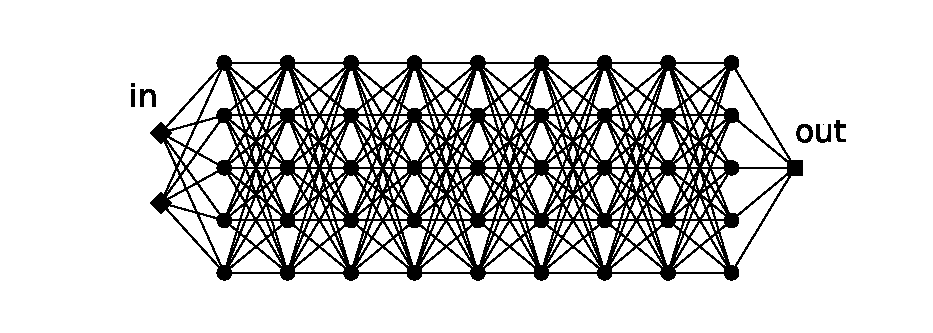
\includegraphics[clip,trim=15mm 5mm 5mm 5mm, scale=0.8]{standardNet2.eps}
\caption{An example of ``narrow'' fully-connected network architecture having $\nu=2$ inputs,   depth $L=9$ and width $H=5$. These architectures provide the optimal approximation rate \eqref{eq:mainineq} with $p=\frac{2}{\nu}$ if $H$ is sufficienly large and held constant while $L$ is increased.}\label{fig:stnet}
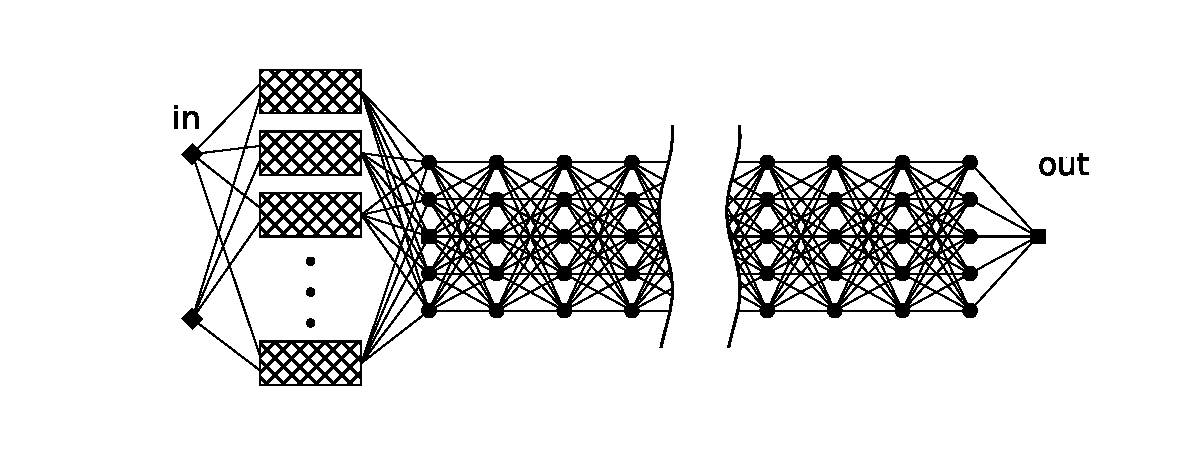
\includegraphics[clip,trim=15mm 5mm 5mm 5mm, scale=0.8]{stackedNet.pdf}
\caption{The ``stacked'' architectures for $p\in(\frac{1}{\nu},\frac{2}{\nu})$, providing the optimal approximation rates \eqref{eq:mainineq} under the depth constraint $L=O(W^{p\nu-1})$.}\label{fig:stackednet}
\end{center}
\end{figure}

We state now our main result as the following theorem.

\begin{theorem}\label{th:main}{}\hfill
\begin{enumerate}
\item[a)] 
For any $p\in (\frac{1}{\nu},\frac{2}{\nu}]$, there exist a sequence of architectures $\eta_W$ with depths $L=O(W^{p\nu-1})$ and respective weight assignments such that inequality \eqref{eq:mainineq} holds with this $p$. 
\item[b)] For $p=\frac{2}{\nu}$, an example of such architectures is the  narrow fully-connected architectures of constant width $2\nu+10$.
\item[c)] For $p\in(\frac{1}{\nu},\frac{2}{\nu})$, an example of such architectures are stacked architectures described above, with the narrow fully-connected subnetwork having width $3^\nu(2\nu+10)$ and depth $W^{p\nu-1}$.
\end{enumerate}
\end{theorem}
Comparing this theorem with Theorem \ref{th:2}a) we see that the narrow fully-connected architectures provide the best possible approximation in the sense of Eq. \eqref{eq:mainineq}. Moreover, for $p\in(\frac{1}{\nu}, \frac{2}{\nu})$ the upper bound on the network depth in Theorem \ref{th:main}c) matches the lower bound in Theorem \ref{th:2}c) up to a logarithmic factor. This proves that for $p\in(\frac{1}{\nu}, \frac{2}{\nu})$ our stacked architectures are also optimal (up to a logarithmic correction) if we additionally impose the asymptotic constraint $L=O(W^{p\nu-1})$ on the network depth.      

We explain now the idea of the proof. Given a function $f$ and some $W$, we first proceed as in Proposition \ref{prop:shallow} and construct its piecewise linear interpolation $\widetilde f_1$ on the length scale $\frac{1}{N}$ with $N\sim W^{1/\nu}$. This approximation has uniform error $O(\omega_f(O(W^{-1/\nu})))$. Then, we improve this approximation by constructing an additional approximation $\widetilde f_2$ for the discrepancy $f-\widetilde f_1$. This second approximation lives on a smaller length scale $\frac{1}{M}$ with $M\sim W^{p}$. In contrast to $\widetilde f_1$, the second approximation is inherently discrete: we consider a finite set of possible shapes of $f-\widetilde f_1$ in patches of linear size $\sim\frac{1}{N}$, and in each patch we use a special single network weight to encode the  shape closest to $f-\widetilde f_1$. The second approximation is then fully determined by the collection of these special encoding weights found for all patches. We make the  parallel subnetwork of the full network serve two purposes: in addition to computing the initial approximation $\widetilde f_1(\mathbf x)$ as in Proposition \ref{prop:shallow}, the subnetwork returns the position of $\mathbf x$ within its patch along with the weight that encodes the second approximation $\widetilde f_2$ within this patch. The remaining, deep narrow part of the network then serves to decode the second approximation within this patch from the special weight and compute the value $\widetilde f_2(\mathbf x)$. Since the second approximation lives on the smaller length scale $\frac{1}{M}$, there are $Z=\exp(O((M/N)^\nu))$ possible  approximations $\widetilde f_2$ within the patch that might need to be encoded in the special weight. It then takes a narrow network of depth $L\sim \ln Z$ to reconstruct the approximation from the special weight using the bit extraction technique of \cite{bartlett1998almost}. As $M\sim W^{p}$, we get $L\sim W^{p\nu-1}$. At the same time, the second approximation allows us to effectively improve the overall approximation scale from $\sim \frac{1}{N}$ down to $\sim \frac{1}{M}$, i.e. to $\sim W^{-p}$, while keeping the total number of weights in the network. This gives us the desired error bound $O(\omega_f(O(W^{-p}))).$ 

We remark that the discontinuity of the weight assignment in our construction is the result of the discreteness of the second approximation $\widetilde f_2$: whereas the variable weights in the network implementing the first approximation $\widetilde f_1$  are found by linearly projecting the approximated function to $\mathbb R$ (namely, by computing $f\mapsto f(\mathbf x)$ at the knots $\mathbf x$), the variable weights for $\widetilde f_2$ are found by assigning to $f$ one of the finitely many values encoding the possible approximate shapes in a patch. This operation is obviously discontinuous.  While the discontinuity is present for all $p>\frac{1}{\nu},$ at smaller $p$ it is ``milder'' in the sense of a smaller number of assignable values.


\section{Discussion}\label{sec:discus}

We discuss now our result in the context of general approximation theory and practical machine learning. First, a theorem of \cite{kainen1999approximation} shows that in the optimal approximations by neural networks the weights generally discontinuously depend on the approximated function, so the discontinuity property that we have established is not surprizing. However, this theorem of \cite{kainen1999approximation} does not in any way quantify the accuracy gain that can be acquired by giving up the continuity of the weights. Our result does this in the practically important case of deep ReLU networks, and explicitly describes a relevant mechanism.  


In general, many nonlinear approximation schemes involve some form of discontinuity, often explicit (e.g., using different expansion bases for different approximated functions (\cite{devore1998nonlinear}). At the same time, discontinuous selection of parameters in parametric models is often perceived as an undesirable  phenomenon associated with unreliable approximation (\cite{devore1989optimal,devore1998nonlinear}). We point out, however, that deep  architectures considered in the present paper resemble some popular state-of-the-art practical networks for highly accurate image recognition -- residual networks \citep{he2016deep} and highway networks \citep{srivastava2015highway} that may have dozens or even hundreds of layers. While our model does not explicitly include shortcut connections as in ResNets, a very similar element is effectively present in the proof of Theorem \ref{th:main} (in the form of channels reserved for passing forward the data). We expect, therefore, that our result may help better understand the properties of ResNet-like networks. 

Quantized network weights have been previously considered from the information-theoretic point of view in \cite{bolcskei2017memory,petersen2017optimal}. In the present paper we do not use quantized weights in the statement of the approximation problem, but they appear in the solution (namely, we use them to store small-scale descriptions of the approximated function). One can expect that weight quantization may play an important role in the future development of the theory of deep networks. 


\section*{Acknowledgments}
The author thanks Alexandr Kuleshov and the anonymous referees for helpful comments and suggestions. The research was supported by the Skoltech SBI Bazykin/Yarotsky project.

\bibliography{relu}

\end{document}